% !TeX spellcheck = en_US
\pagetarget{Campaign}{\addsection{Campaign Rules}{\spells/town_portal.png}}

\begin{multicols*}{2}

A campaign is a series of scenario designed for solo play.

\subsection*{Starting a Scenario}
At the start of each campaign scenario, set your income by placing your Faction cubes on the following spaces of the income tracker on the Town board:
\begin{multicols}{3}
  \centering
  \LARGE
  10~\svg[14]{gold}

  \columnbreak
  0~\svg[14]{building_materials}

  \columnbreak
  0~\svg[14]{valuablegreater}
\end{multicols}
Special rules in each scenario can change the above values.

Campaigns have unique bonuses that \textbf{replace} the regular starting bonus from the chosen \pagelink{Difficulty}{Difficulty}.

Prepare AI Enemies: their \pagelink{AI Heroes}{units} and their \pagelink{AI Deck}{AI decks}.

\subsection*{Finishing a Scenario}
After finishing a \textbf{Solo Campaign} Scenario, reset your Hero's Experience Level to 1, and prepare the starting Deck for the next Scenario of the campaign.
It will consist of:
\begin{itemize}
  \item all the \pagelink{Statistic}{Statistic} cards from your Deck,
  \item the Level I \pagelink{Specialty}{Specialty} card,
  \item 5 other non-Specialty cards of your choice from your Deck.
\end{itemize}
Skip \pagelink{Setup Starting Deck}{steps 11--13 of Setup} for the next Scenario of the campaign.

Note down the list of cards in your starting Deck.
If you lose the Scenario, reset the Deck to the same list.

\note{6}{If your Hero is at some point given a Spell, Artifact, or Ability card that is unavailable, \textbf{Search (3)} the respective card's deck to get another card in its stead.}

\subsection*{Using different Heroes}
Although each campaign has its own recommended Hero for whom it is balanced and who is also the main character of the story, you are free to play with any other Hero of the same Faction.

If you choose to change your Hero between the Scenarios or when you repeat the scenario with a different Hero,
replace all of the previous Hero’s Statistic cards and the level I Specialty card with all of the Statistic cards and the level I Specialty card of your new Hero.
If the previous Hero had \pagelink{Empowered Statistic}{Empowered Statistics cards},
you can remove Statistic cards of the same type from the new Hero’s deck, and replace them with Empowered Statistic cards of the corresponding type.
You can replace any card in the ``5 other non-Specialty cards'' group with new Hero’s starting Ability card (if you don't already have a copy of that Ability) and Magic Arrow(s).
You cannot have more than 4 Magic Arrow cards.
% TODO if the old hero had 5 magic arrows, do I need to remove one?

\vspace*{\fill}

\columnbreak
\pagetarget{AI Heroes}{\subheader{AI Heroes}}
AI Heroes are used in the Campaigns.
Their units are static and are defined by the Scenario: find the indicated unit cards when you start the scenario.
If the unit indicates unit tier (\svg{bronze}, \svg{silver}, \svg{golden}, or \svg{azure}) instead of ``Few'' or ``Pack'', that's a Neutral Unit.

During setup, if multiple AI Heroes use the same unit, and you do not have enough copies of its card, the AI Heroes must share it -- set everything up without that card, and add it to the AI Hero's Army the moment you trigger Combat with them.

AI Heroes cannot surrender and you cannot surrender to them;
they will always fight until they run out of units.
Winning Combat against an AI Hero does not grant any rewards unless stated by the Scenario.
AI Heroes do not have a Town Board, Resources, or a Hero Board.

\subsection*{AI Turns}
Unless specified otherwise, AI heroes start in their Town, take turns after the player, and have 3 MP, always spending them to perform the following Actions in descending priority:
\begin{itemize}
  \item If a player's Hero is on the same Tile as the AI, spend all MP to move towards them in an attempt to start Combat.
  \item If there are any Mines or Settlements the AI could flag on the same Tile, move towards the closest one.
  \item Otherwise, move toward the player's Town.
Repeat this sequence until all MPs are used up.
AI Heroes take their turn after the player.
\end{itemize}

AI Heroes always \textbf{automatically win Combat} against any Neutral Units, while simultaneously \textbf{flagging or Visiting all Fields} they happen to move through.
They gain no benefits from any Fields.

AI Heroes must discover face down Map Tiles as normal by spending 1 MP before moving onto them.
The player chooses that Tile's orientation.

\end{multicols*}

\pagetarget{AI Deck}{\subheader{AI Decks}}
\begin{multicols*}{2}
\begin{multicols*}{2}
  \begin{center}
    \vspace*{-1.5em}
    \begin{tikzpicture}
      \draw (0, 0) node {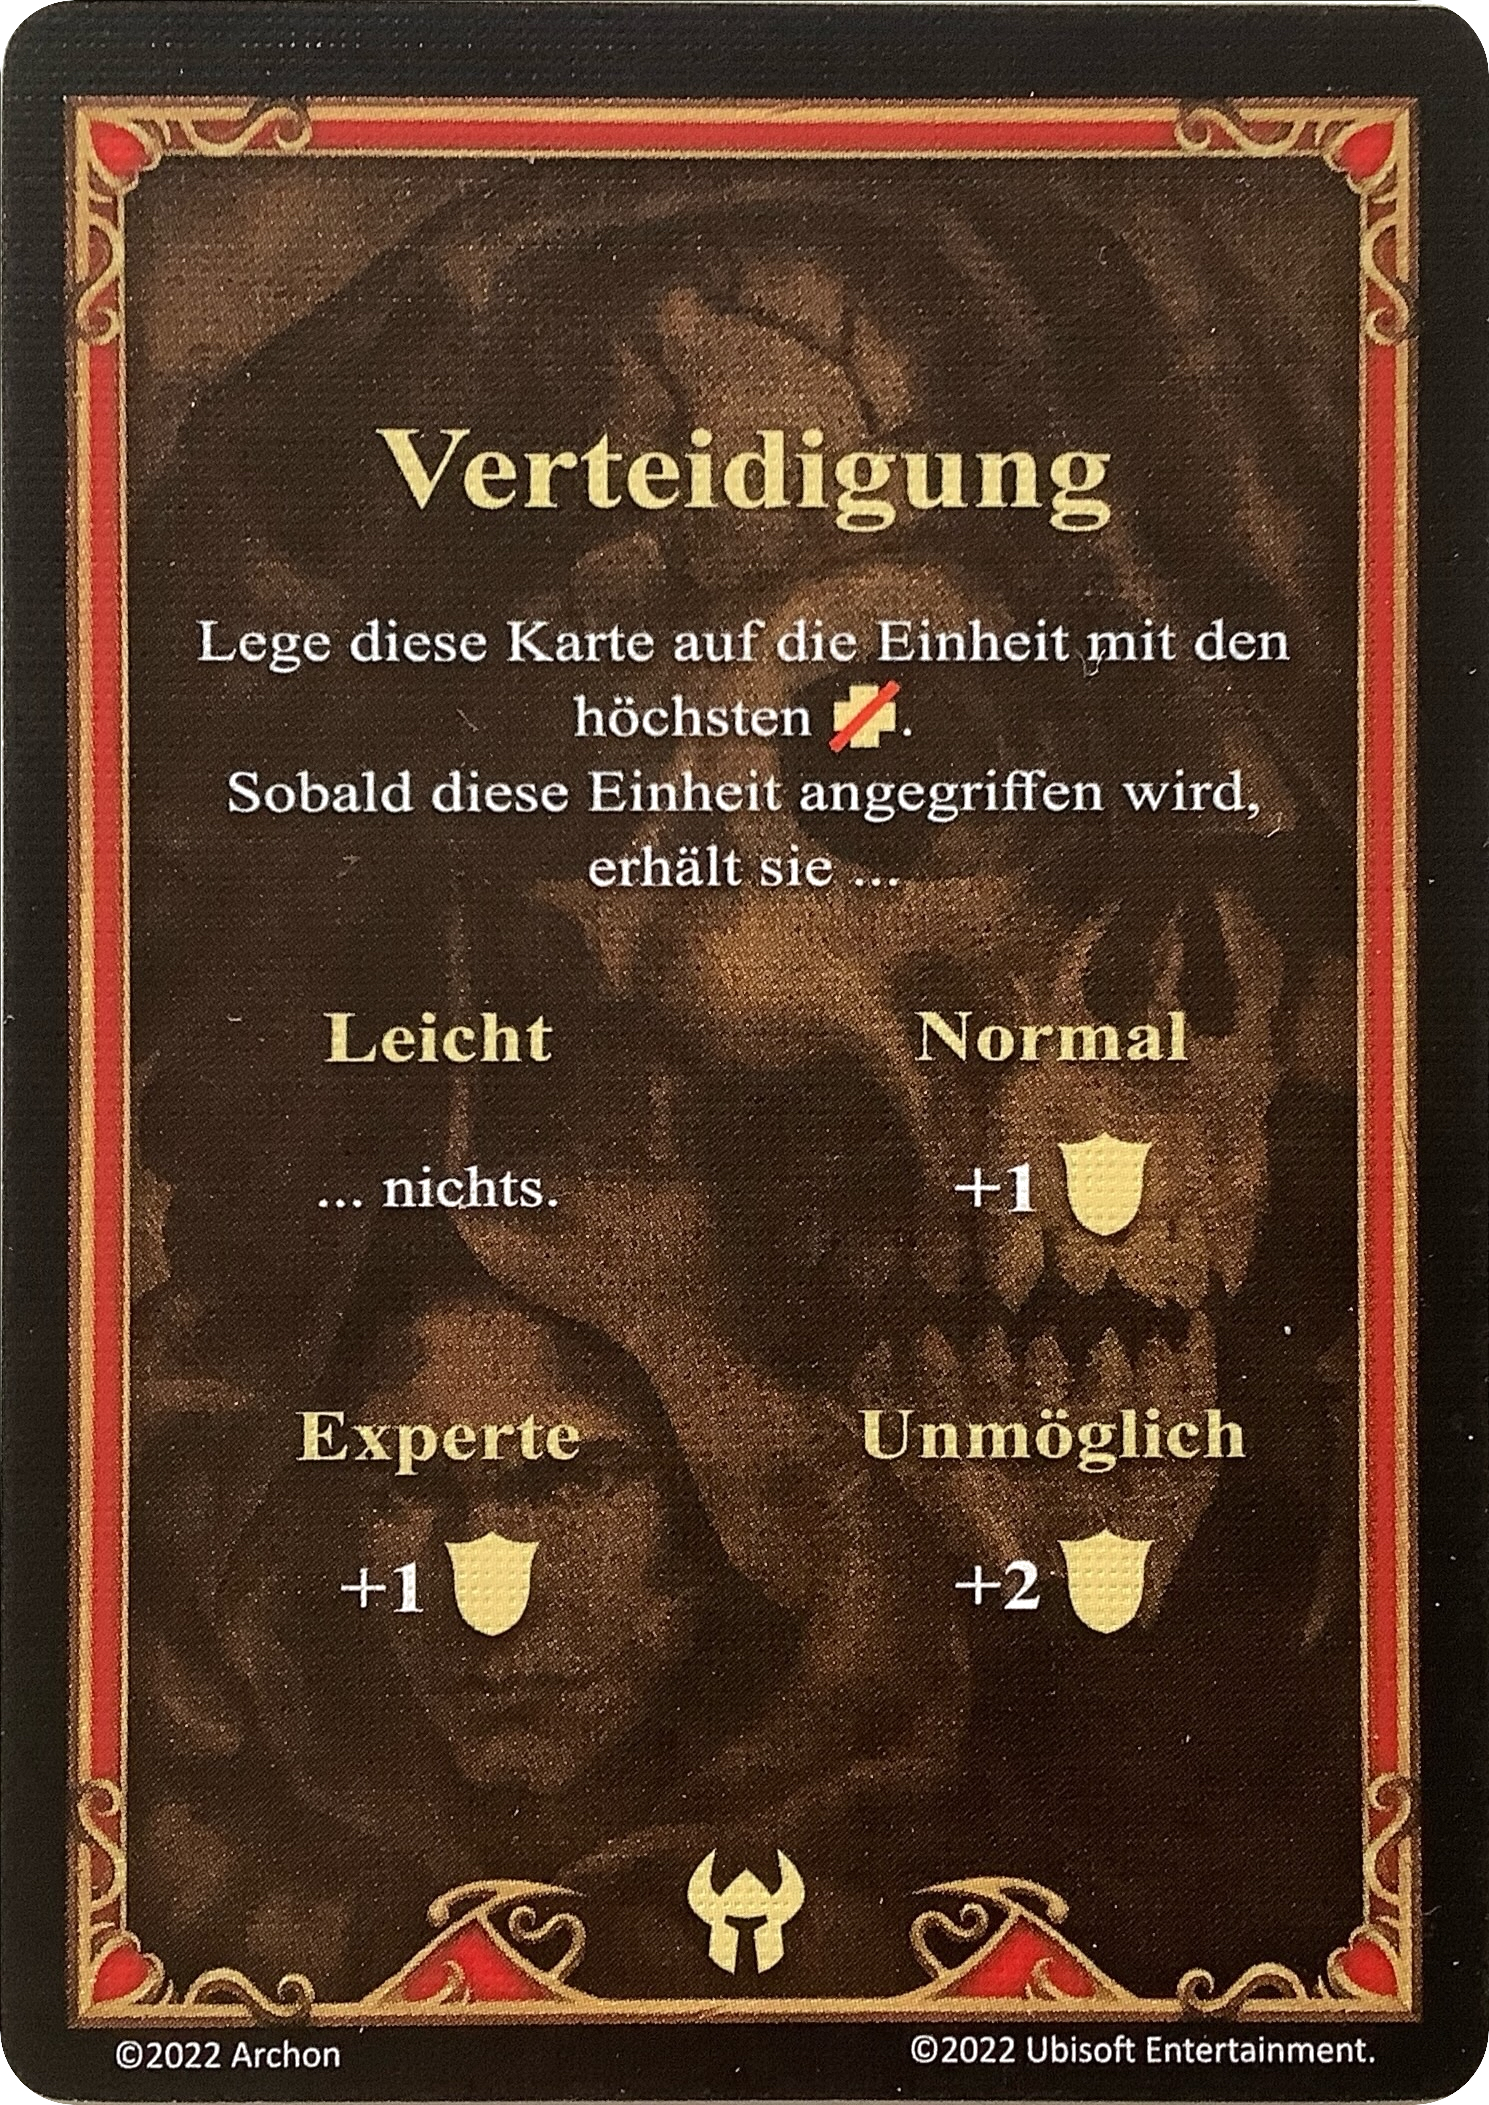
\includegraphics[width=1.3\linewidth]{\cards/ai.png}};
      \draw (-0.7, 2.5) node {\encircle{1}};
      \draw (1.5, 1.2) node {\encircle{2}};
      \draw (-1.5, 0) node {\encircle{3}};
      \draw (0.5, 0) node {\encircle{4}};
      \draw (-1.5, -1.2) node {\encircle{5}};
      \draw (0.5, -1.2) node {\encircle{6}};
      \draw (-0.5, -2.5) node {\encircle{7}};
    \end{tikzpicture}\\
    \phantom{\ldots\ldots}\imagecaption{AI card}
    \vspace*{-1em}
  \end{center}
  \vspace*{\fill}
  \columnbreak
  \scriptsize
  \begin{itemize}[itemsep=0pt]
    \item[\textbf{1.}] Name
    \item[\textbf{2.}] Description
    \item[\textbf{3.}] Easy Modifier
    \item[\textbf{4.}] Normal Modifier
    \item[\textbf{5.}] Expert Modifier
    \item[\textbf{6.}] Impossible\\Modifier
    \item[\textbf{7.}] Card Type:\\\svg{might}, \svg{magic}, or \svg{skill}
  \end{itemize}\vspace*{\fill}
\end{multicols*}

AI Heroes use two Decks during Combat: the \textbf{AI Deck}, and the \textbf{AI Spell Deck}.
The AI Deck consists of three types of AI cards: Might \svg[12]{might}, Magic \svg{magic} and Skill \svg{skill}.
Each Campaign Scenario lists the number and types of cards to include during setup.
Choose these cards \textbf{randomly} when building the AI Deck.
Shuffle the AI Deck before each Combat together with its discard pile.

When an AI Hero \textbf{activates} a unit, draw an AI card\index{AI card} and follow its instructions before the unit \pagelink{AI Units}{moves and/or attacks}.
If AI Deck is depleted during Combat, stop drawing from it.
The effect of each AI card depends on the game's \pagelink{Difficulty}{Difficulty}.
If an AI Hero is instructed to draw a card, they will draw and resolve \textbf{another card} from the AI Deck.

If an AI card increased a unit's \svg{defense}, or triggered another card which increased it, the AI card stays attached to the unit until the first defense happens.
% TODO: why attack isn't mention in expansion book? is it not the case for attack?
% our old text here: The Might card \svg[12]{might} is attached to the unit until the first respective attack/defense happens.

\subsection*{AI Deck sharing}
If there are multiple AI Enemy Armies in the Scenario, but the rules don't specify which Enemy an AI Deck, an AI Spell Deck, or a Skill belongs to, you should assume it is shared between them.

\subsection*{AI Magic \svg{magic} cards and AI Spell Deck}
Build the \textbf{AI Spell Deck} by separating the indicated Spells from the regular Spell Deck during setup.
Shuffle the AI Spell Deck before each Combat together with its discard pile.

Whenever an AI Magic card \svg{magic} is drawn, draw the next spell from the the AI Spell Deck, and cast it.
Discarded spells go to its own AI Spell Discard pile.
If the AI Spell deck empties before Combat ends, shuffle the AI Spell discard pile to form a new Spell deck.

Sometimes in the AI Spell deck, there are more Spell cards than there are Magic cards in the AI Hero's deck.
This is no mistake: not all spells need to be used, some are there for the sake of diversity.

If the AI Hero is assigned a Spell card that is unavailable because it's your Hero's Deck, and you don't have another copy, substitute it with a \wikilink{spells/magic_arrow}{Magic Arrow} card.

\subsection*{AI Skill \svg{skill} cards}
% TODO need rephrasing to better disambiguate the AI Skill card with the \svg{skill} symbol vs the Ability card assigned to the hero
If Skill cards are included, search for and set aside the indicated card related to it (usually, an Ability).
Whenever an AI Hero uses the skill assigned to them in the Setup, do not discard it afterwards.
Contrary to the regular rules, the AI Hero can use the skill again, when instructed to do so by the AI deck.

AI Skill cards cannot be replaced, so if setup assigns the AI Hero a card that your Hero has and you don't have another copy,
remove the needed card from your Hero's deck and \textbf{Search (3)} the respective card's deck to compensate your Hero for the loss.

\end{multicols*}
